\chapter{Tópicos de gerenciamento de requisitos}

\section{Rastreabilidade de requisitos}

Segundo Sayão(2005), o rastreamento de requisitos é utilizado para prover os relacionamentos entre os requisitos, arquitetura e a implementação final dos mesmos no sistema, ele permite uma compreensão adequada do dos relacionamentos de dependência dos requisitos desde o nível mais alto até o nível mais baixo, na questão de arquitetura e implementação ele utiliza dos artefatos para gerar essa rastreabilidade.
Para realizar essa rastreabilidade de requisitos são utilizadas várias técnicas, porém nesse trabalho a equipe vai trabalhar com a rastreabilidade horizontal e vertical.

\subsection{Rastreabilidade Horizontal}
Segundo Dall'Oglio, essa rastreabilidade está relacionada com a habilidade de relacionar artefatos entre diferentes modelos, dentre esses artefatos podem estar requisitos, artefatos de análise, de design, entre outros.


\begin{figure}[!htpb]
\centering
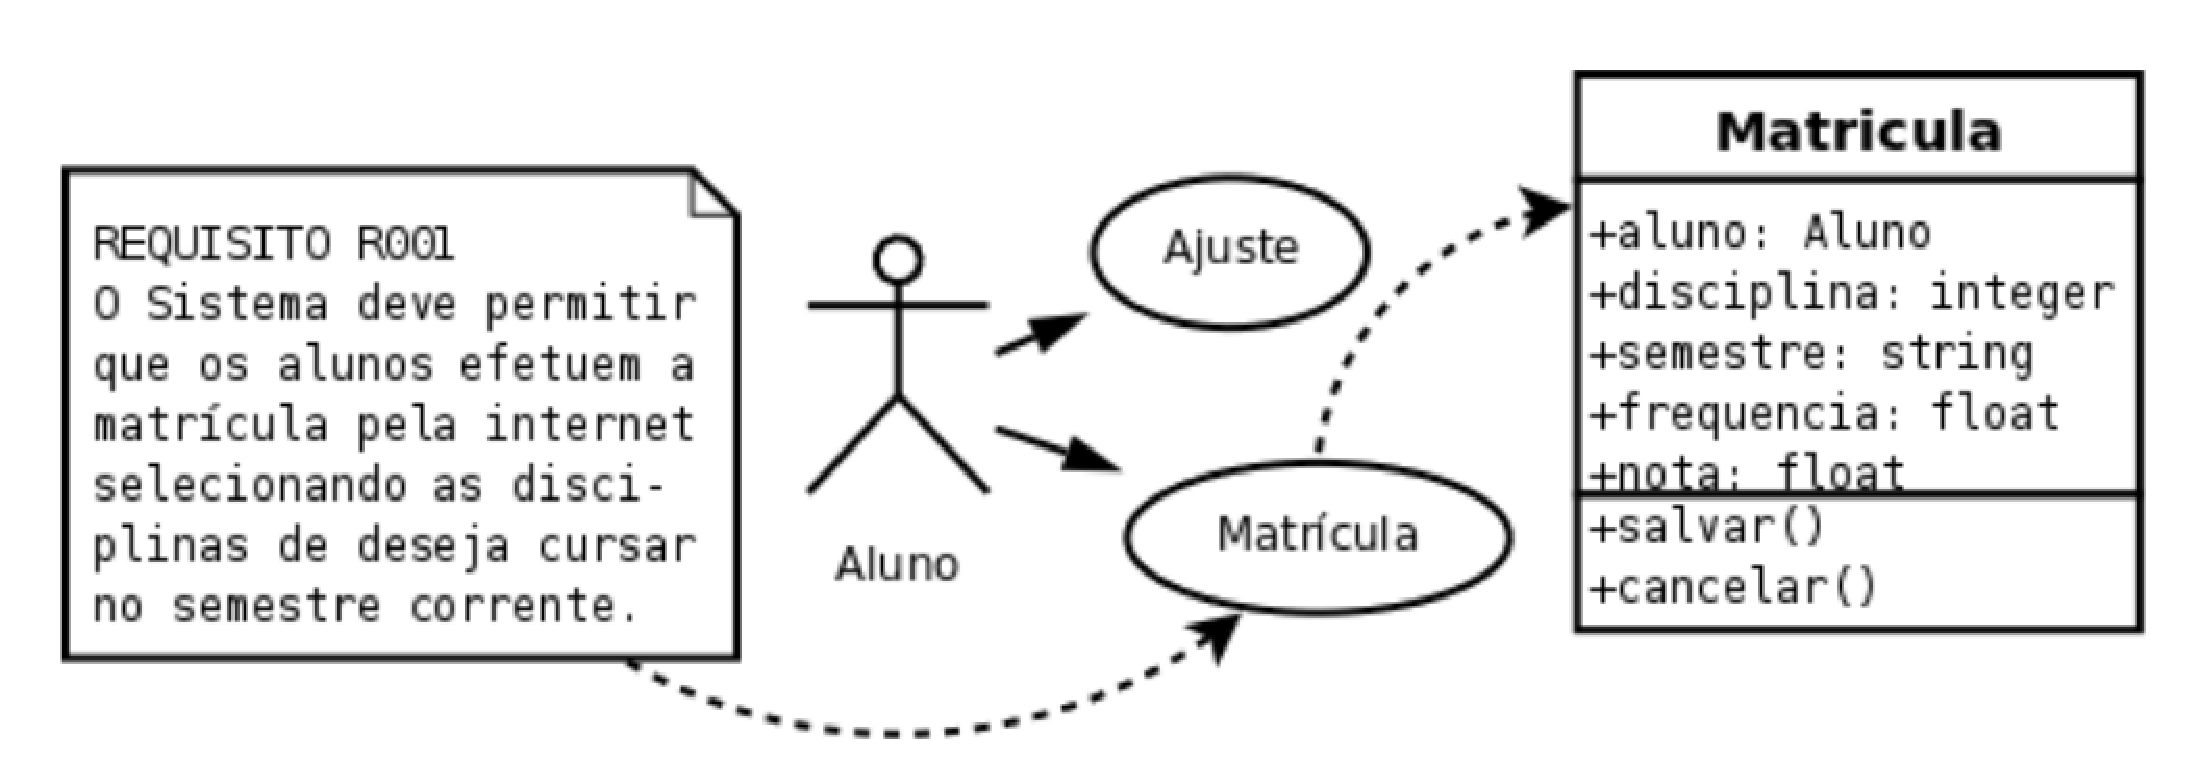
\includegraphics[scale=0.4]{figuras/gerenciamento/horizontal}
\caption{Exemplo de rastreabilidade horizontal retirado do artigo de Dall'Oglio}
\end{figure}

\subsection{Rastreabilidade Vertical}
Segundo Dall'Oglio, a rastreabilidade vertical está relacionada com a capacidade de detectar relacionamento entre artefatos dependentes dentro de um modelo de processo utilizado.

\begin{figure}[!htpb]
\centering
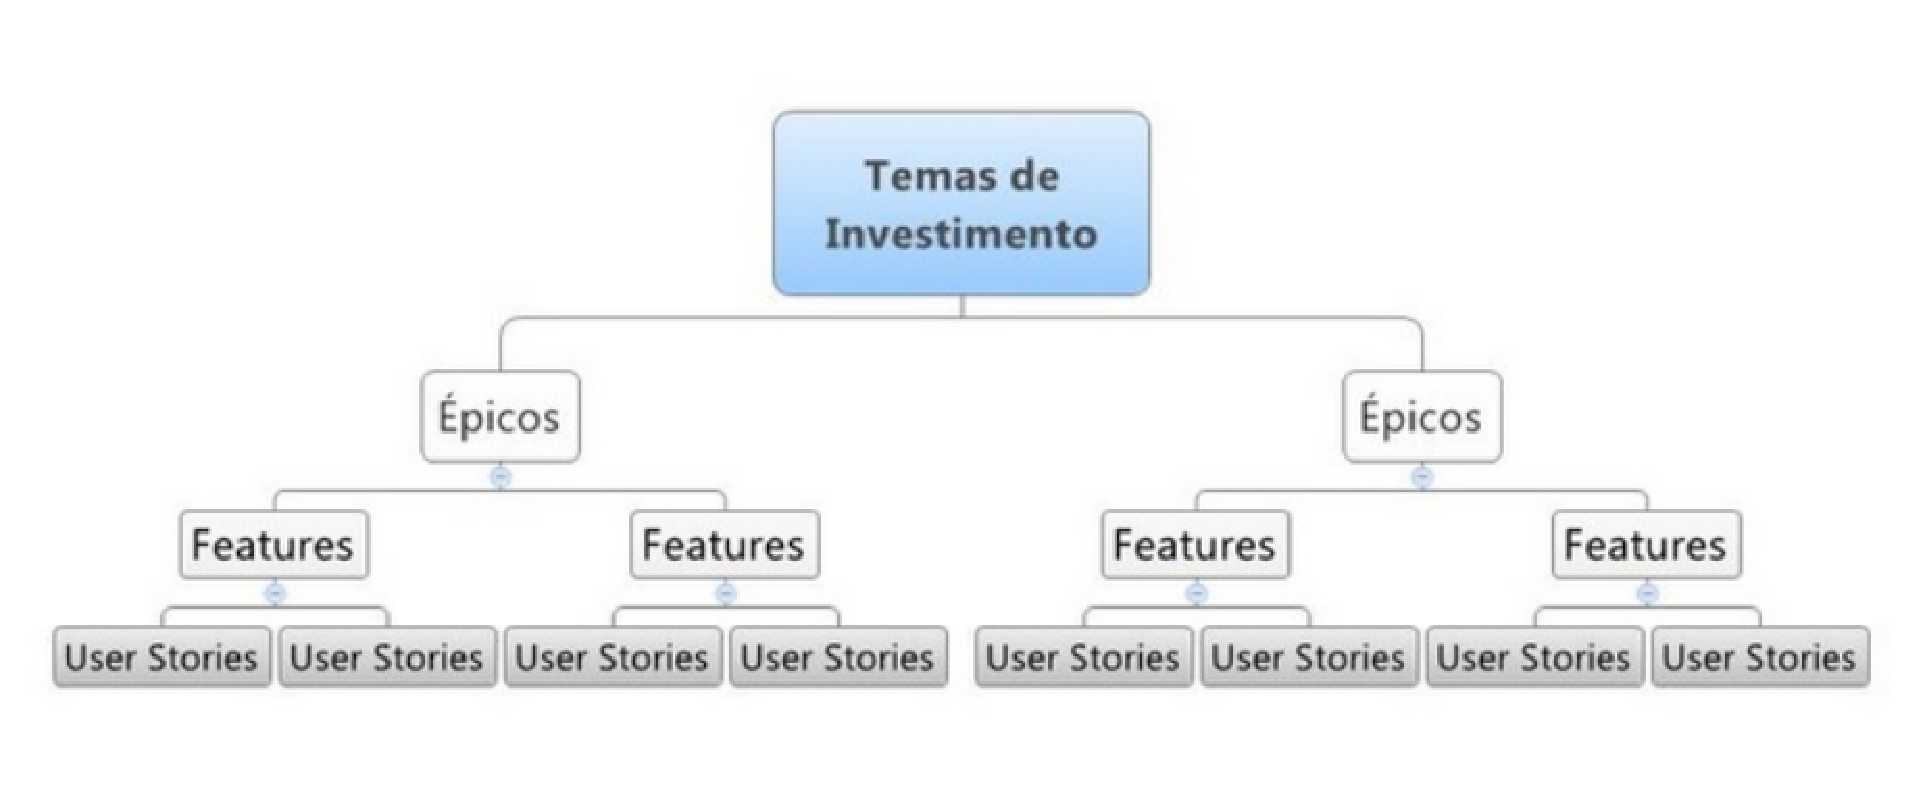
\includegraphics[scale=0.4]{figuras/gerenciamento/vertical}
\caption{Exemplo de rastreabilidade vertical}
\end{figure}

\newpage
\section{Atributos de requisitos}

Os atributos dos requisitos são as prioridades de um requisito, além de deixarem mais claros os requisitos, eles podem ser utilizados para fornecer informações significativas sobre o estado atual do sistema.  
Existem vários tipos de atributos para requisitos, os que vão ser utilizados no trabalho são:
\begin{itemize}
\item Origem: Pessoa, documento que foi a influência na criação de tal requisito, útil para determinar onde tirar dúvidas sobre o requisito, ou realizar um agrupamento por fontes.
\item Prioridade: Declaração da importância do requisito em relação ao sistema, ou a outros requisitos, podendo variar de Crítico, Importante a Opcional.
\begin{itemize}
\item Crítico: Sem esse requisito o sistema não entra em funcionamento e o desejo do cliente não é atendido.
\item Importante: Sem esse requisito o sistema funciona, mas ainda não satisfaz todas as necessidades do cliente.
\item Opcional: A falta desse requisito não vai influenciar nas necessidades do cliente, seria algo que iria agregar valor, mas não é tão importante.
\end{itemize}

\item Atribuído a: Quem na equipe irá indicar que o requisito foi satisfeito.
\item Data de criação: Data em que o requisito foi criado na ferramenta.
\item Data de início: Data planejada pela equipe para dar início a implementação do requisito.
\item Data de conclusão: Data planejada pela equipe para finalizar a implementação do requisito.
\item Dificuldade: A quantidade de esforço que aquele requisito vai demandar da equipe, na abordagem adotada a equipe utilizará do sistema de Planning Poker com uso da sequência de Fibonacci para definir a dificuldade através de pontos. No Planning Poker, os pontos de um requisito só são definidos quando todos os membros da equipe estão de acordo.
\item Status: É o estado atual do requisito, podendo variar de Novo, Em desenvolvimento a Feito. A parte de progresso pode ser dividida em subpartes de estado, tais como Elicitado, em Progresso, em Teste e Feito.

\item Risco: É a medida de certeza sobre o impacto que um requisito pode ter sobre um sistema. Pode variar entre Alto, Médio ou Baixo.
\begin{itemize}
\item Alto: Indica que o impacto é significativo para o andamento do desenvolvimento sistema.
\item Médio: Os impactos são grandes, mas não tão significativos para o andamento do desenvolvimento do sistema.
\item Baixo: Os impactos são mais leves, ou não tem influência sobre o desenvolvimento do sistema.
\end{itemize}
\end{itemize}